\documentclass[handout]{beamer}
\usetheme[]{Szeged}
\usecolortheme{beaver}
\setbeamertemplate{footline}[frame number]
\usepackage[utf8]{inputenc}
\usepackage[spanish,es-nodecimaldot]{babel}
\usepackage{amsmath, amsthm, amsfonts, amssymb}
\usepackage{textcomp}
\usepackage{multimedia}
\DeclareGraphicsExtensions{.png,.pdf,.jpg,.jpeg}
\graphicspath{{imagenes/}} %directorio donde se guardan las imagenes
\usepackage{hyperref}

% \renewcommand{\footnotesize}{\small}
% \renewcommand*{\bibfont}{\scriptsize} 
% \renewcommand{\bibfont}{\normalfont\small}

\title{Calor y temperatura}
\author{Bloque II}
\institute[FC UNAM]{Preparatoria \\ Universidad del Valle de México}
% \logo{
\includegraphics[width=1.2cm]{uvm}}
\date{\today}

\begin{document}
\frametitle{La temperatura}

\begin{frame}[noframenumbering]
  \titlepage
  \begin{center}
    
\includegraphics[width=5.5cm]{uvm1}    
  \end{center}  
\end{frame}


\section{Calor y temperatura}


\begin{frame}
  \frametitle{El calor}


  \begin{block}{¿Qué es el calor?}
    En el siglo XVII creían que era un fluido invisible, sin sabor, olor ni peso, al que
    llamaban \textbf{calórico}. Sólo conocian los efectos, entre más caliente estaba un objeto más
    calórico tenía.
  \end{block}


  \begin{center}
    \begin{figure}[h]
      \centering
      
\includegraphics[scale=0.08]{ghost}
    \caption{¡Consideraban al calórico como si fuera un fantasma!}
  \end{figure}
  \end{center}
  
  Actualmente el \textbf{calor} se interpreta como \textbf{la energía en tránsito que fluye de
    objetos de mayor temperatura a objetos de menor temperatura}.
  
\end{frame}



\begin{frame}
  \frametitle{La temperatura}
  \begin{block}{¿Qué es la temperatura?}
    La temperatura es un magnitud física que indica qué tan caliente o fría está una
    sustancia y se mide con un termómetro.
  \end{block}

  \begin{itemize}
  \item Nuestro cuerpo no detecta la temperatura, si no las variaciones de calor.
  \item Al cambiar la temperartura de un objeto pueden cambiar sus propiedades físicas.
  \item Es uno de los parámetros que describen un sistema. Los otros son la presión y el
    volumen
  \item Es una propiedad intensiva. 
  \end{itemize}
\end{frame}

\begin{frame}
  \begin{figure}[h]
    \centering
    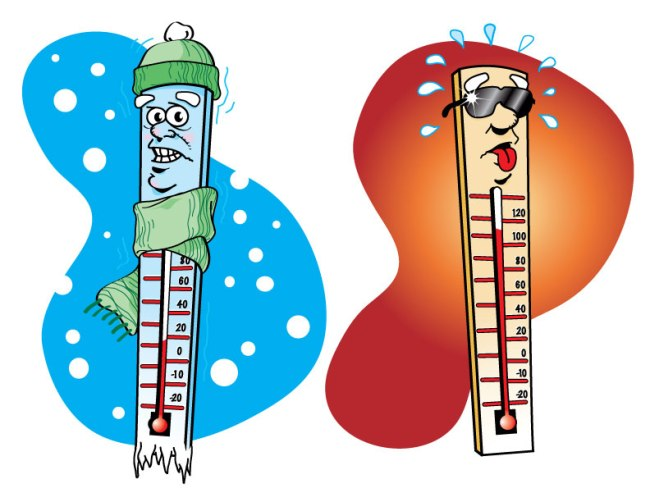
\includegraphics[scale=0.3]{temperature}
  \end{figure}

  \begin{center}
    \huge
    ¡La temperatura y el calor están relacionados pero no son lo mismo!
  \end{center}
\end{frame}


\begin{frame}
  \frametitle{Medición de la temperatura}
  \begin{block}{Termómetro}
    \begin{itemize}
    \item Es el instrumento que mide la temperatura
    \item Para conocer el valor de la temperatura de un objeto, necesita estar en
      \textbf{equilibrio térmico} con el termómetro.
    \item Usa el fenómeno de dilatación en los fluidos.
    \item Con los termómetros de \texttt{Hg}, se pueden medir temperaturas dentro de un
      rango de -39 \textdegree C a 357 \textdegree C.
    \end{itemize}
  \end{block}
  \begin{center}
    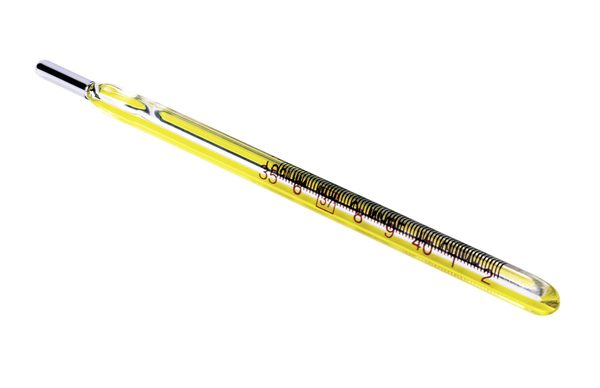
\includegraphics[width=4cm]{termometro}
  \end{center}
\end{frame}


\begin{frame}
  \frametitle{Escalas de temperatura y sus unidades}
  \begin{itemize}
  \item Fahrenheit
  \item Celsius
  \item Kelvin
  \item Rankine
  \end{itemize}


\end{frame}


\begin{frame}
  \frametitle{Escala Farenheit}
  \begin{center}
    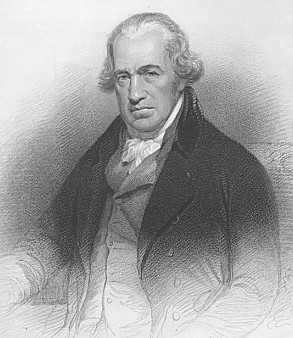
\includegraphics[width=3cm]{farenheit}
  \end{center}
  \begin{itemize}
  \item Nacio en Polonia en el año de 1686 y murio en Holanda en 1736.
  \item Soplador de vidrio y fabricante de instrumentos.
  \item Desarrollo el termómetro de mercurio.
  \item El motivo para asignar 96 medidas entre la temperatura de la mezlca fría y su
    cuerpo. Fue obtener una escala formada por una docena de divisiones cada una compuesta
    por 8 partes. 
  \end{itemize}
\end{frame}

\begin{frame}
  \frametitle{Escala Celsius}
  \begin{center}
    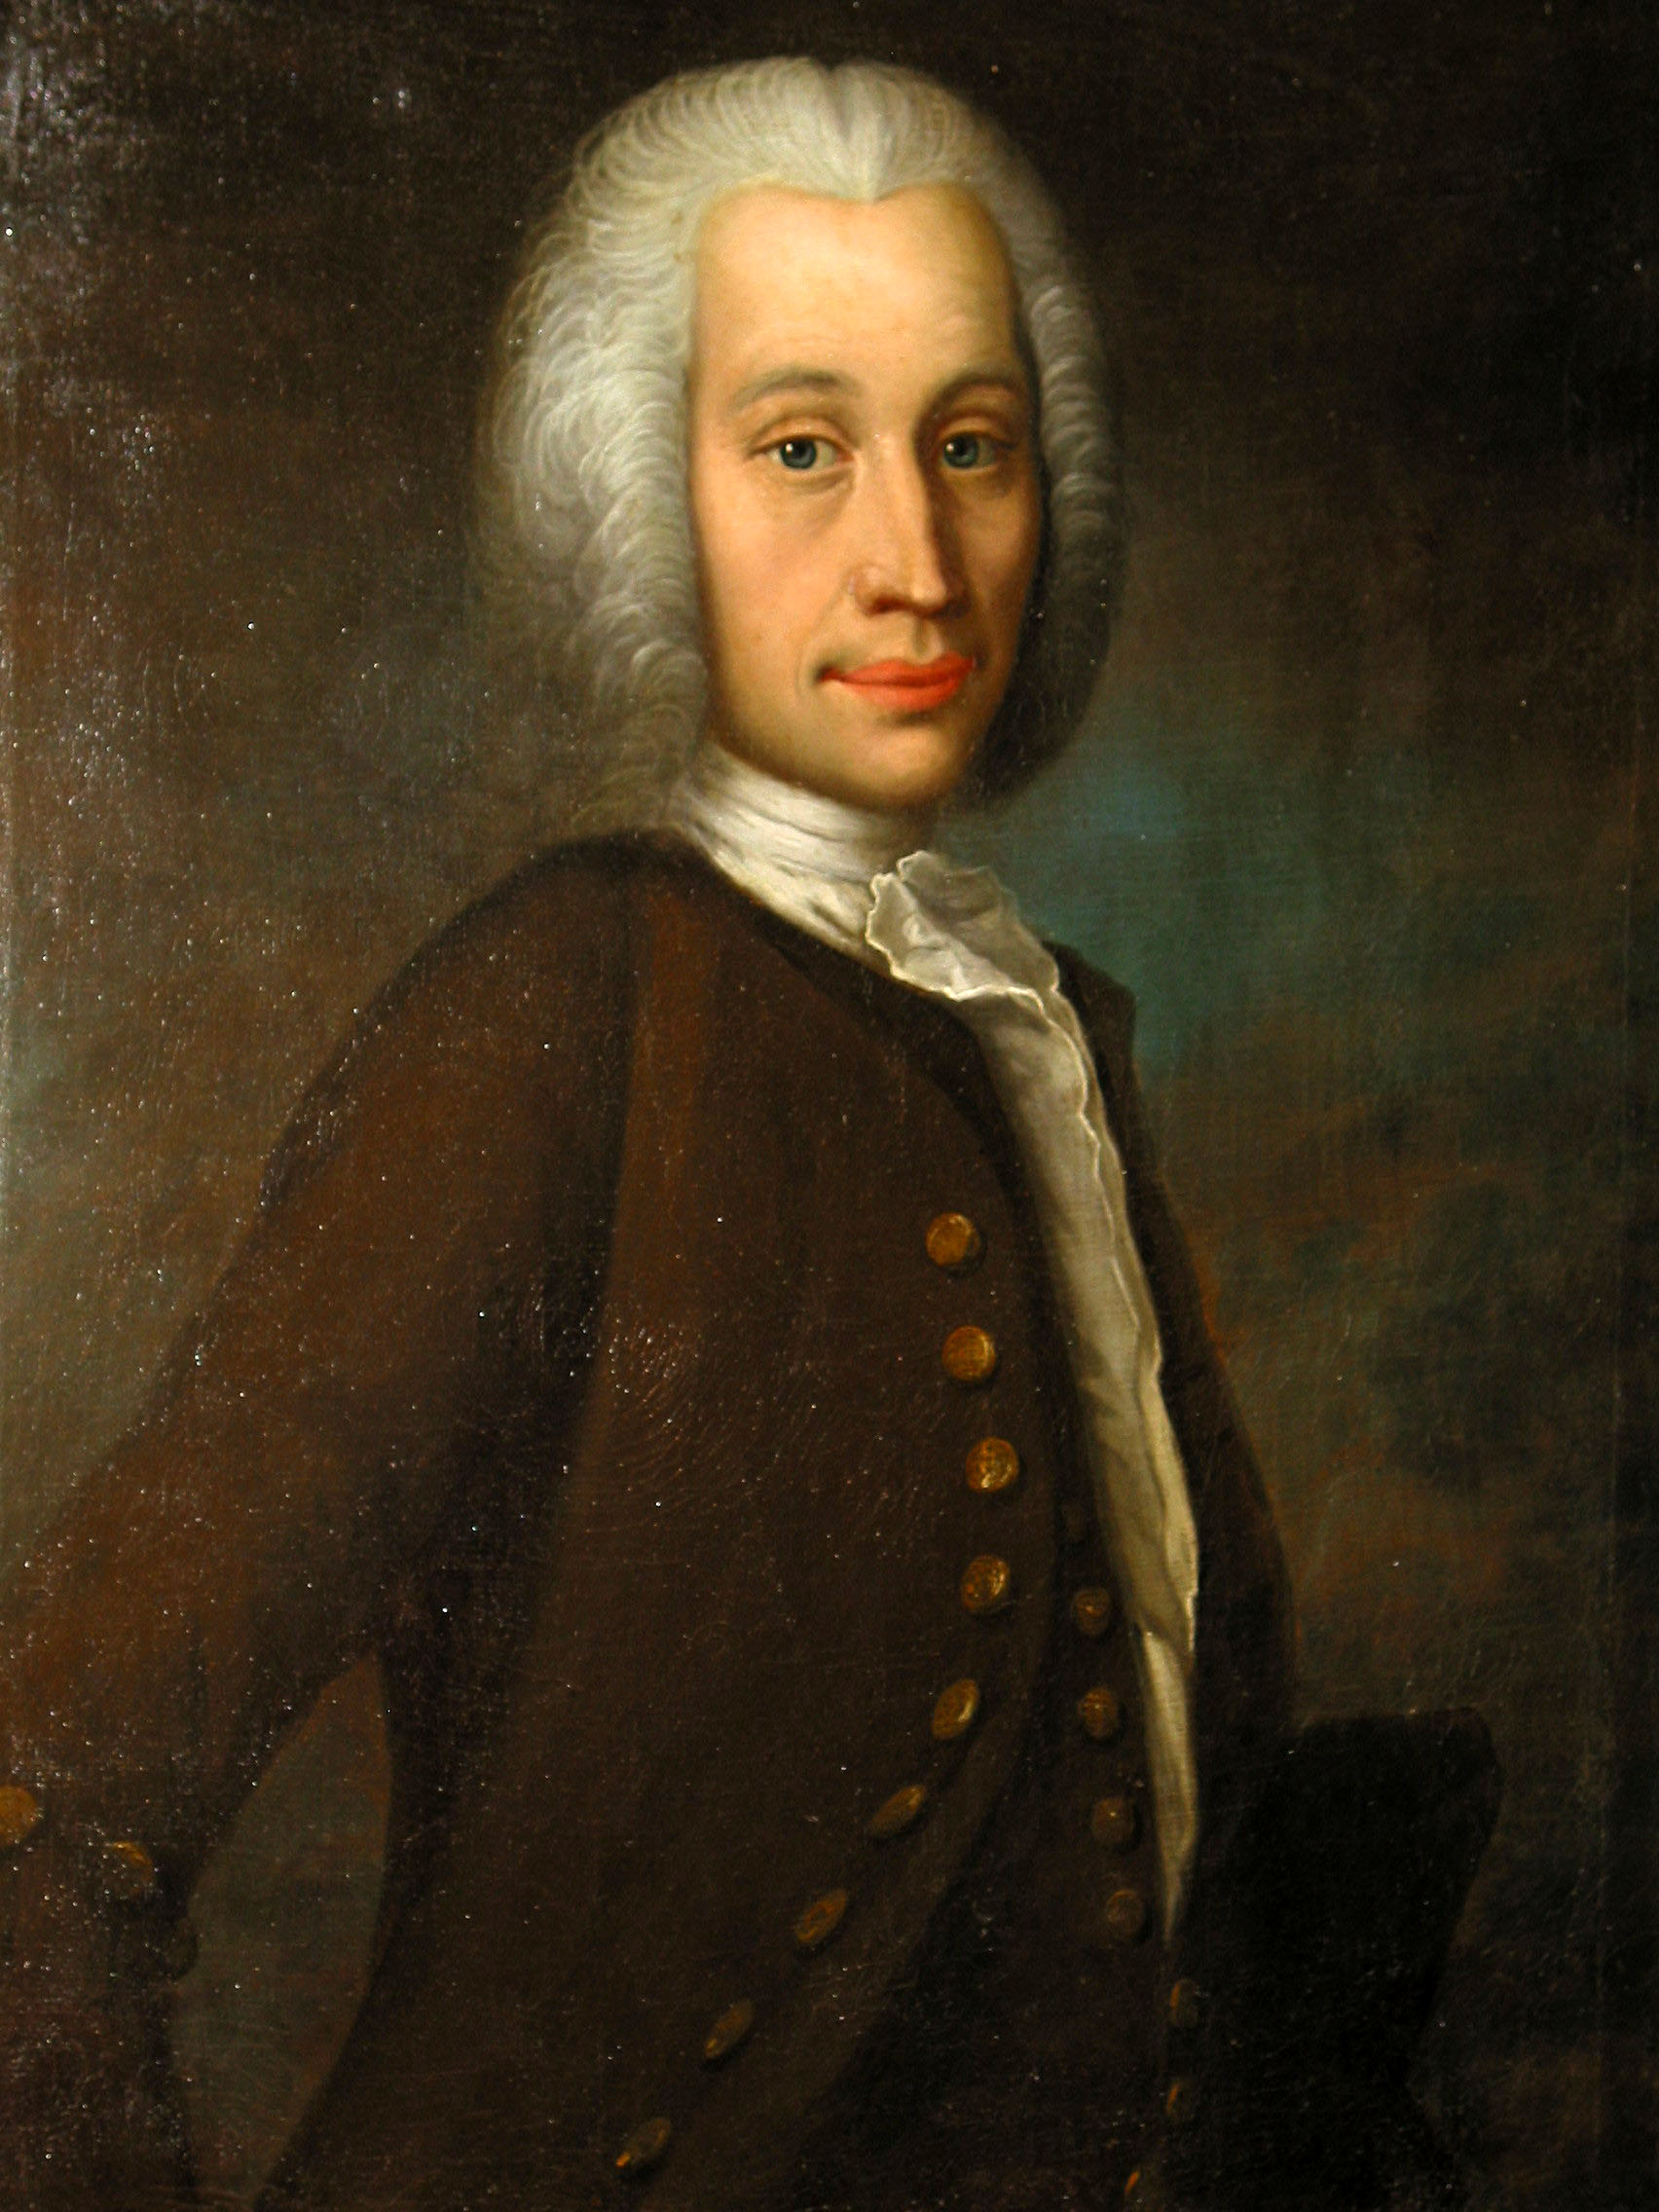
\includegraphics[width=3cm]{celsius}
  \end{center}

  \begin{itemize}
  \item Nació en Suecia en 1701 y murió en el mismo país en 1744.
  \item Astrónomo, físico, matemático, geólogo.
  \item Director del Observatorio de Upsala, Suecia.
  \end{itemize}
\end{frame}

\begin{frame}
  \frametitle{Escala Rankine}
  \begin{center}
    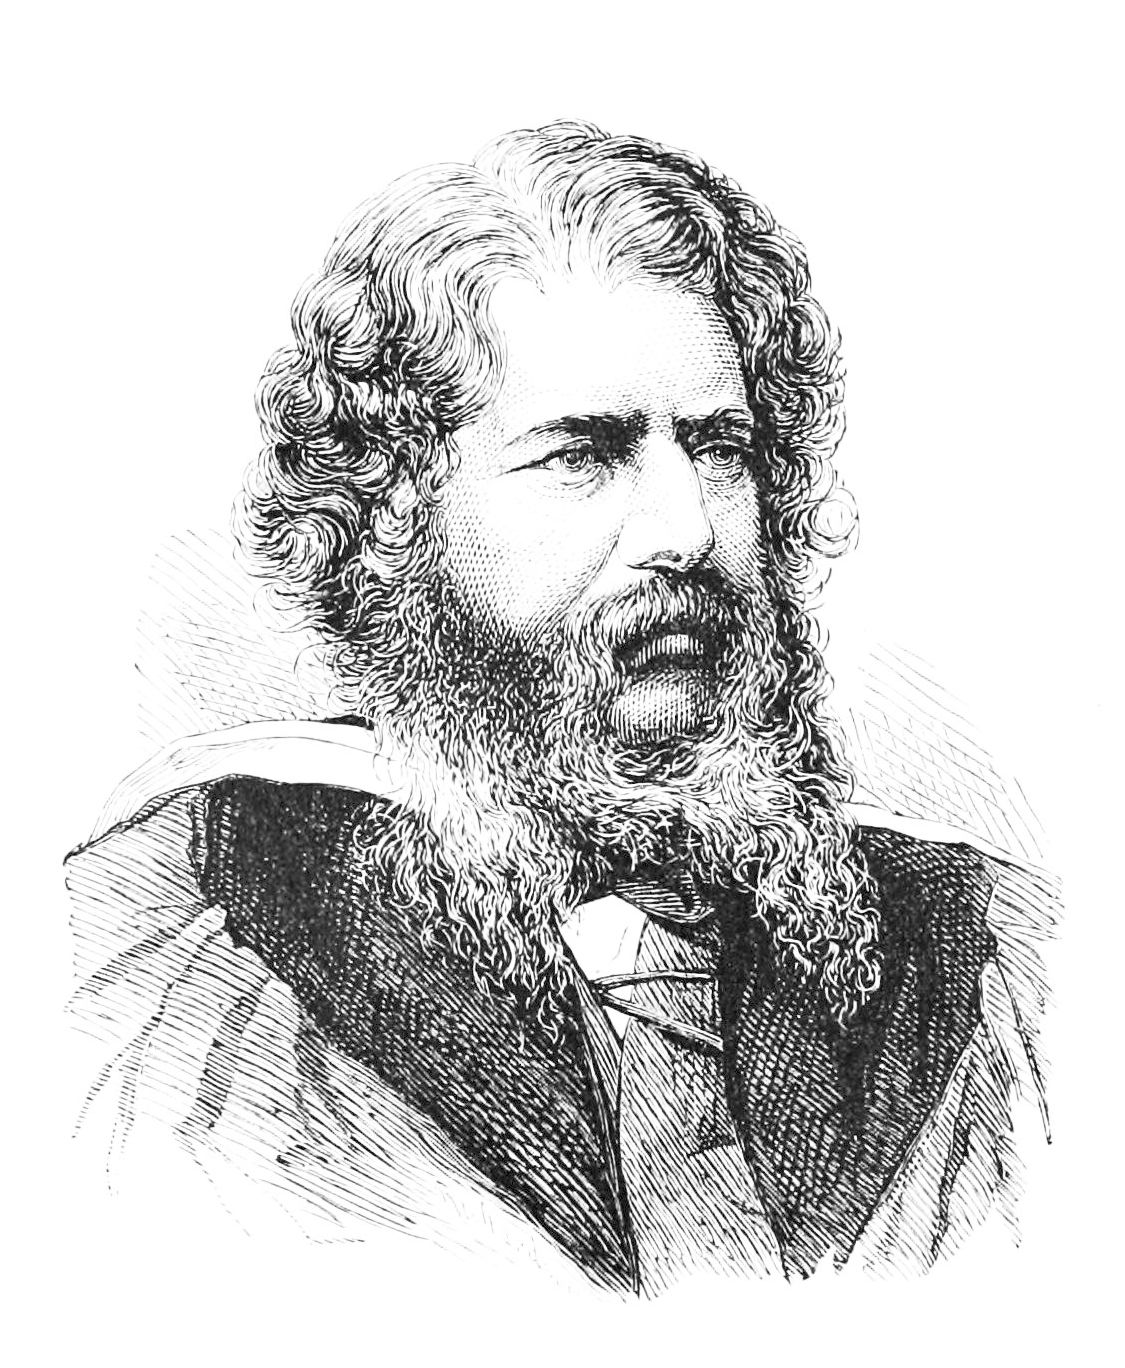
\includegraphics[width=3cm]{rankine}
  \end{center}

  \begin{itemize}
  \item Ingeniero y físico escoses.
  \item Nació en 1820 y murió en 1872.
  \item Pionero de la teoría termodinámica junto con, R. Clausius y Lord
    Kelvin.
  \end{itemize}
\end{frame}

\begin{frame}
  \frametitle{Escala Kelvin}
  \begin{center}
    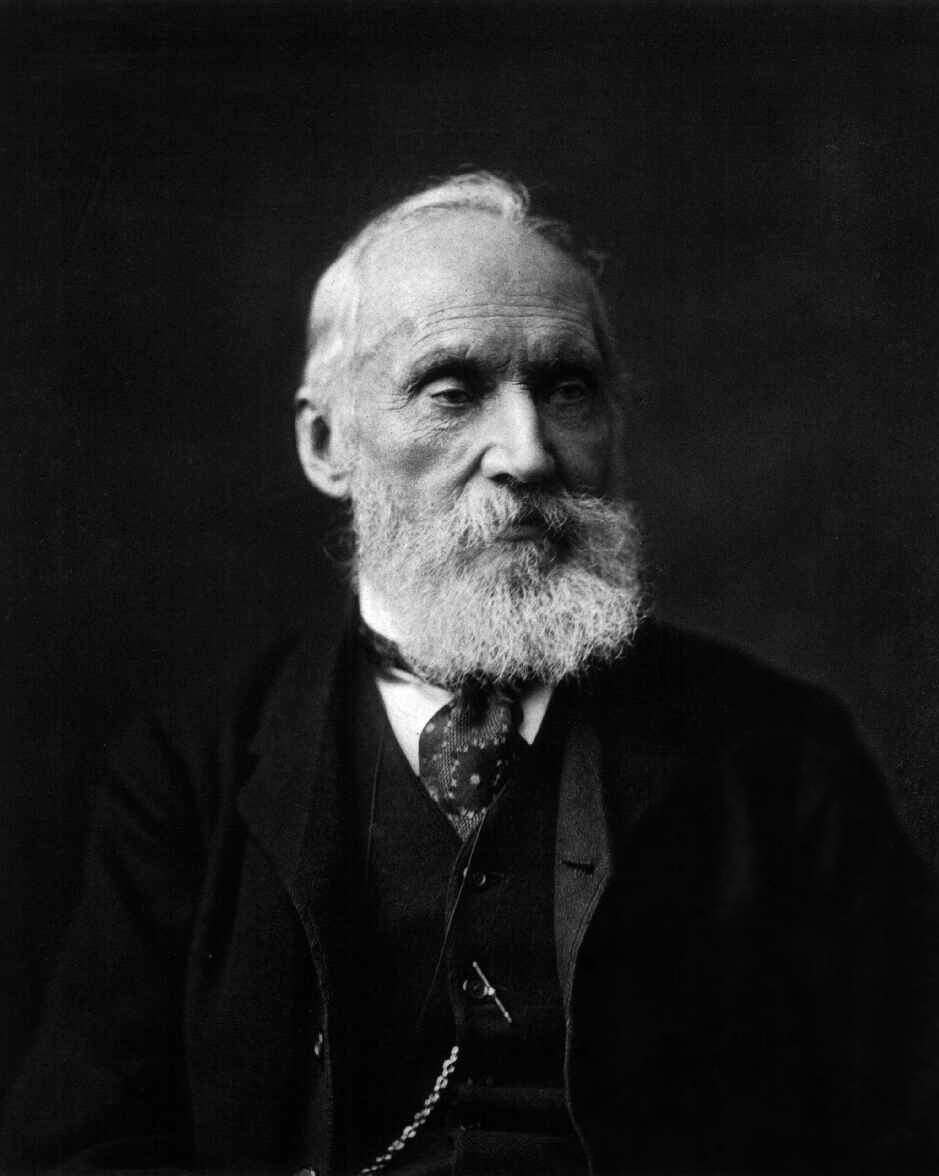
\includegraphics[width=3cm]{kelvin}
  \end{center}

  \begin{itemize}
  \item Físico y matemático británico. (1824-1870)
  \item Su verdadero nombre es William Thompson.
  \item Es la unidad de medida de temperatura del Sistema Internacional de Unidades.
  \item A los 0 K se le denomina cero absoluto, Donde los átomos y moleculas tienen la
    mínima energía posible. 
  \end{itemize}
\end{frame}

\begin{frame}
  \frametitle{Transformación de temperaturas de una escala a otra}
  \begin{block}{Transformación entre Kelvin y Celsius}
    \begin{tabular}{ccl}
      K & = & \textdegree C + 273 \\
      \textdegree C & = & K - 273 \\
    \end{tabular}
  \end{block}

  \begin{block}{Transformación entre Celsius y Fahrenheit}
    \begin{tabular}{ccl}
      \textdegree F & = & 1.8\textdegree C + 32 \\
      \textdegree C & = & $\frac{\mbox{\textdegree F }-32}{1.8}$ \\
    \end{tabular}
  \end{block}

  \begin{block}{Transformación entre Rankine y Fahrenheit}
    \begin{tabular}{ccl}
      \textdegree R & = & \textdegree F + 460 \\
    \end{tabular}
  \end{block}
\end{frame}

\begin{frame}
  \frametitle{Comparación entre escalas}
  \begin{center}
    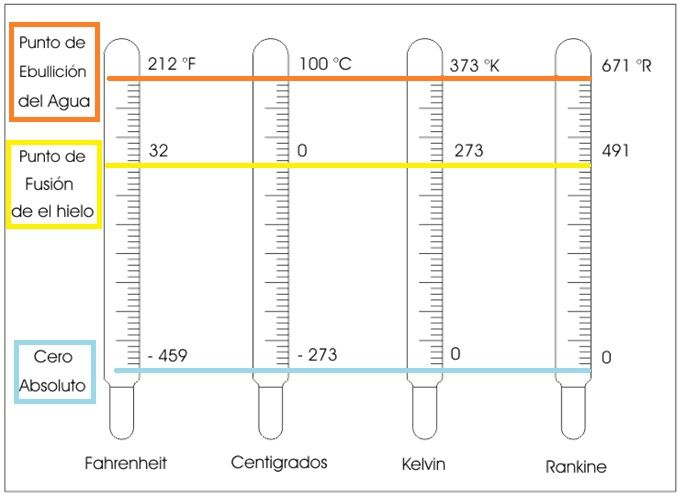
\includegraphics[scale=0.45]{comparacion}
  \end{center}
\end{frame}

\begin{frame}
  \frametitle{Más sobre el concepto de calor}
  \begin{itemize}
  \item El calor es energía en tránsito.
  \item Un cuerpo no posee calor si no energía interna, el calor es la energía calorífica.
  \item La energía interna se define com la suma de las energías potencial y cinética de todas
    las moléculas que los constituyen.
  \item Todo objeto debido a su temperatura tiene la capacidad de transferir energía
    calorífica a otro objeto o sistema que se encuentre a más baja temperatura.
  \end{itemize}
\end{frame}


\begin{frame}
  \begin{center}
    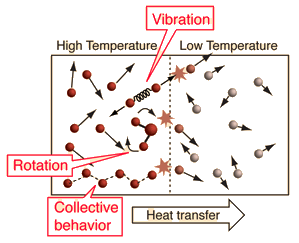
\includegraphics[width=5cm]{templowhigh1}
    \newline
    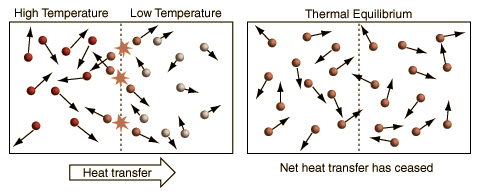
\includegraphics[width=8cm]{templowhigh}
  \end{center}
\end{frame}





\begin{frame}
  \frametitle{Unidades de medida del calor}
Las unidades de medida del calor son las mismas que las unidades del trabajo mecánico y de
la energía.
\begin{block}{Unidades de calor}
  joule = Newton metro = Nm = J
\end{block}



Para medir el calor de manera práctica se usan unidades como:
\begin{description}
\item[Caloría:] Cantidad de calor aplicado a un gramo de agua para elevar su temperatura 1
  \textdegree C, de 14.5 a 15.5 \textdegree C.
\item[Kilocaloría:] 1000 \texttt{cal} equivalen a 1 \texttt{kcal}.
\item[BTU:] Cantidad de calor aplicada a una libra de agua (454 g) para elevar su
  temperatura en un grado Fahrenheit.
\end{description}

\begin{block}{Equivalencia de unidades}
  \begin{tabular}[h]{ccc}
    1 joule & = & 0.24 cal \\
    1 caloría & = & 4.2 J \\
  \end{tabular}
\end{block}
\end{frame}


\begin{frame}
  \frametitle{Mecanismos por medio de los cuales el calor se transmite de un cuerpo a
    otro}
  \begin{block}{}
    A nivel molecular el equilibrio térmico es porque la energía cinética media o promedio
    de sus moleculas es igual.
  \end{block}

  \begin{block}{}
    \textbf{El calor siempre se transmite de objetos de mayor temperatura a objetos de menor
      temperatura.}
  \end{block}
  % \movie[width=3cm,height=2cm,poster]{}{cat.mp4}
  \begin{itemize}
  \item Conducción
  \item Convección
  \item Radiación
  \end{itemize}
  
\end{frame}


\begin{frame}[allowframebreaks,t]
  \frametitle{Actividad}
Convertir a la escala pedida.
  \begin{itemize}
  \item 0 \textdegree C a Kelvin
  \item 230 \textdegree F a Celsius
  \item 0 K a Celsius
  \item -30 \textdegree F a Celsius
  \item 100 \textdegree F a Kelvin
  \item 373 K a Celsius
  \item 800 \textdegree C a Fahrenheit
  \item 100 R a Fahrenheit
  \item -100 Celsius a Kelvin
  \item 0 \textdegree F a Celsius
  \end{itemize}
% \end{block}
% \end{frame}

% \begin{frame}
\begin{block}{Investigar}
  \begin{itemize}
  \item Investigar que formas transmición del calor existen y explicar cada una de ellas brevemente.
  \item En TUS propias palabras escribe la diferencia entre calor y temperatura. Da un
    ejemplo.
  \item ¿Por qué los alimentos cocinados en aceite llegan a ser más sabrosos que los
    cocinados en agua?
  \end{itemize}
\end{block}

\end{frame}



\begin{frame}
  \frametitle{Conducción}
  
\end{frame}


% \begin{frame}
%   \frametitle{Conducción}
  
% \end{frame}

% \begin{frame}
%   \frametitle{Convección }
  
% \end{frame}


% \begin{frame}
%   \frametitle{Radiación}
  
% \end{frame}

\section{Dilatación térmica}

\begin{frame}
  \frametitle{Dilatación térmica}

  dialatación lineal
  coeficiente de dilatación lineal
  Consideraciones practicas acerca de la dilatación
\end{frame}


\section{Calor específico}


\section{Procesos termodinámicos}


Problemas





\end{document}